\documentclass[12pt]{article}

\usepackage{answers}
\usepackage{setspace}
\usepackage{graphicx}
\usepackage{enumitem}
\usepackage{multicol}
\usepackage{mathrsfs}
\usepackage[margin=1in]{geometry} 
\usepackage{amsmath,amsthm,amssymb}
\usepackage[english]{babel}

\newcommand{\N}{\mathbb{N}}
\newcommand{\Z}{\mathbb{Z}}
\newcommand{\C}{\mathbb{C}}
\newcommand{\R}{\mathbb{R}}

\DeclareMathOperator{\sech}{sech}
\DeclareMathOperator{\csch}{csch}

\newenvironment{theorem}[2][Theorem]{\begin{trivlist}
		\item[\hskip \labelsep {\bfseries #1}\hskip \labelsep {\bfseries #2.}]}{\end{trivlist}}
\newenvironment{definition}[2][Definition]{\begin{trivlist}
		\item[\hskip \labelsep {\bfseries #1}\hskip \labelsep {\bfseries #2.}]}{\end{trivlist}}
\newenvironment{proposition}[2][Proposition]{\begin{trivlist}
		\item[\hskip \labelsep {\bfseries #1}\hskip \labelsep {\bfseries #2.}]}{\end{trivlist}}
\newenvironment{lemma}[2][Lemma]{\begin{trivlist}
		\item[\hskip \labelsep {\bfseries #1}\hskip \labelsep {\bfseries #2.}]}{\end{trivlist}}
\newenvironment{exercise}[2][Exercise]{\begin{trivlist}
		\item[\hskip \labelsep {\bfseries #1}\hskip \labelsep {\bfseries #2.}]}{\end{trivlist}}
\newenvironment{solution}[2][Solution]{\begin{trivlist}
		\item[\hskip \labelsep {\bfseries #1}]}{\end{trivlist}}
\newenvironment{problem}[2][Problem]{\begin{trivlist}
		\item[\hskip \labelsep {\bfseries #1}\hskip \labelsep {\bfseries #2.}]}{\end{trivlist}}
\newenvironment{question}[2][Question]{\begin{trivlist}
		\item[\hskip \labelsep {\bfseries #1}\hskip \labelsep {\bfseries #2.}]}{\end{trivlist}}
\newenvironment{corollary}[2][Corollary]{\begin{trivlist}
		\item[\hskip \labelsep {\bfseries #1}\hskip \labelsep {\bfseries #2.}]}{\end{trivlist}}

\begin{document}
	
	% --------------------------------------------------------------
	%                         Start here
	% --------------------------------------------------------------
	
	\title{IT-Security}%replace with the appropriate homework number
	\author{Michael Gabler} %if necessary, replace with your course title
	
	\maketitle
	
	\section{Definitions}
	
	\textbf{C-I-A Triad}
	\begin{enumerate}
		\item \textbf{C}onfidentiality: prevents unauthorized access to private data
		\item \textbf{I}ntegrity: protects information from being modified by unauthorized parties
		\item \textbf{A}vailability: authorized parties have access to the information when needed
		\item \textbf{A}uthenticity: Being able to verify a party
		\item \textbf{A}ccountability: To guaranty that a property or action belongs to one specific entity
	\end{enumerate}
	\textbf{Security Threat} A potential for violation of security (interruption (a), interception (p), modification (a), fabrication (a) of information) $\rightarrow$ splits up into active and passive\\
	\textbf{Security Attack} Action that compromises the security of information\\
	\textbf{Security Mechanism} A process or device that is designed to detect, prevent or recover from a security attack\\
	\textbf{Security Service} Service to prevent security attacks by implementing one or more mechanisms\\
	\textbf{Co-prime} are two numbers $a$ and $b$ when $\gcd(a,b) = 1$
	
	\section{One Key Cryptography}
	\textbf{Kerckhoffs' principle} \textit{The enemy knows the system} $\rightarrow$ The cipher should remain secure if the adversary knows the specification of the cipher\\
	$\Rightarrow$ not respecting this principle means \textbf{security by obscurity}\\
	\textbf{Encryption Scheme} is a pair of encryption ($Enc$) and decryption ($Dec$) algorithm with $Dec_k(Enc_k(m)) = m$ for every plaintext message $m \in M$ plaintext space and key $k \in K$ key space. $Dec_k(m) = c$ generates the cipher $c \in C$ ciphertext space.\\
	\textbf{Security of an encryption scheme} The adversary should not learn any additional information about $m$ when receiving $c$
	
	\subsection{Historical ciphers}
	\paragraph{Caesar's shift cipher} $M = {A,...,Z} = {0,...,25}$ words over alphabet\\
	$K = {0,...25}$\\
	$Enc_k(m_0,...,m_n) = (k+m_0 mod 26,..., k+m_n mod 26)$\\
	$Dec_k(c_0,...,c_n) = (c_0-k mod 26,..., c_n-k mod 26)$\\
	$\Rightarrow$ can be broken by brute force attack (try every key) since $|K| = 26$
	\paragraph{Substitution cipher}
	Do not shift each letter with the same key but use a mapping table\\
	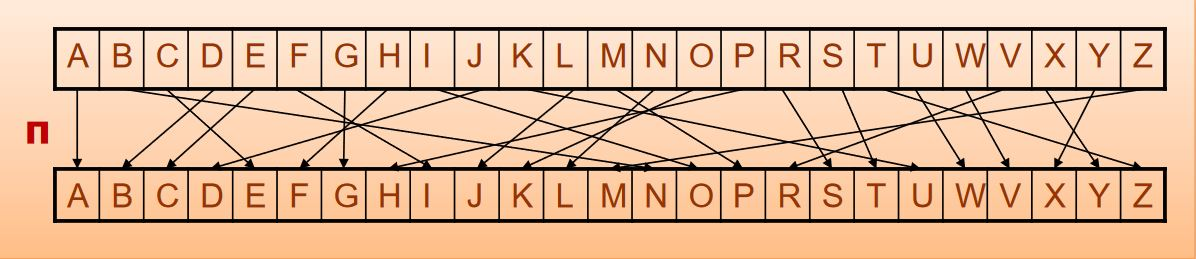
\includegraphics[width=\textwidth]{figures/substitution-cipher.JPG}\\
	$\Rightarrow$ can be broken by using statistical patterns: for example the letter E is the most frequent in the german language
	\paragraph{Vigenère cipher} Use a key with arbitrary length of letters. Each letter of the key defines the shift value for a plaintext letter. If the plaintext is longer than the key it must be repeated.\\
	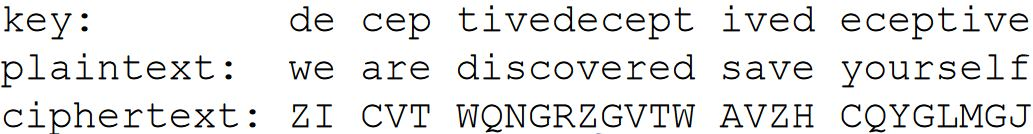
\includegraphics[width=\textwidth]{figures/vigenere-cipher.JPG}\\
	$\Rightarrow$ when the key is repeated its possible that the same letters are encrypted with the same shift which result in the same ciphertext. If such \textbf{identical parts} are found the \textbf{length of $k$} can be computed. Now it's possible to break the cipher by applying $|k|$-times the \textbf{frequency attack} from the substitution cipher.
	
	\subsection{One-time pad}
	$K = M = C = {0,1}^t$\\
	$Enc_k(m) = k xor m$\\
	$Dec_k(m) = k xor c$\\
	$\Rightarrow$ This is perfectly secure but not practical because a key can only be used once (otherwise same ciphertext for same plaintext) and therefore must be as long as the message which is also not practical. So there's no other perfectly secret cipher.\\
	$\Rightarrow$ Other encryption schemes rely on a limitation of the adversary's power (mostly meant \underline{computational} power)
	\textbf{Computational security} A system $X$ is $(t,\epsilon)$-secure if every Turing Machine that operates in time $t$ can break it with probability at most $\epsilon$ where $\epsilon$ is negligible (close to 0).
	
	\subsection{Attacks}
	\textbf{Ciphertext-only attack} The adversary has no information about the plaintext\\
	\textbf{Known plaintext attack} The plaintext is drawn from some distribution that the adversary does not control\\
	\textbf{Chosen-plaintext attack} The adversary can choose arbitrary plaintext and receives the ciphertext from it\\
	\textbf{Chosen-ciphertext attack} The adversary gets information by receiving the decryption of chosen ciphertexts
	
	\subsection{Modern cryptography}
	\textbf{One-way functions} are functions that are poly-time computable and hard to invert. Rely on a mathematical hardness assumption.\\
	\textbf{Pseudorandom generators (PRG)} Generate bits that look random. Depens on a seed (for example system time). Can be constructed by using a one-way function. They are cryptographic if it's not % TODO finish definition\\
	\textbf{Stream cipher} cipher with an infinite stream of bits as output (for example RC4 used for WEP, WPA) $\rightarrow$ PRGs are stream ciphers\\
	\textbf{Block ciphers} are almost equal to pseudorandom permutations (PRP) (permutation is pseudorandom if it can't be distinguished from a real random permutation). Block ciphers permute a predefined amount of plaintext or data into a ciphertext of the same length. Popular block ciphers are:\\
	\begin{tabular}{|l|c|c|}
		\hline 
		& \textbf{key length} & \textbf{block length} \\ 
		\hline 
		DES (Data Encryption Standard) & 56 & 64 \\ 
		\hline 
		IDEA (International Data Encryption Algorithm) & 128 & 64 \\ 
		\hline 
		AES (Advanced Encryption Standard) & 128, 192 or 256 & 128 \\ 
		\hline 
	\end{tabular}\\
	\textbf{Padding} If a stream encrypted with a block cipher the last plaintext block needs to be padded (for example PKCS\#5: add $x$ bytes with value $x$)
	
	\subsubsection{Modes of operation}
	They describe how large amounts of plaintext can be encrypted using block ciphers.\\
	\begin{tabular}{|l|c|c|c|c|}
		\hline 
		& ECB & CBC & OFB & CTR \\ 
		\hline 
		error in $c_i$ affects & $c_i$ & $c_i$, $c_{i+1}$ & $c_i$ & $c_i$ \\ 
		\hline 
		parallel encryption & yes & no & no & yes \\ 
		\hline 
		parallel decryption & yes & yes & no & yes \\ 
		\hline 
		change 1 bit of $m_i$ & $c_i$ & all & $c_i$ & $c_i$ \\ 
		\hline 
	\end{tabular}

	\paragraph{Electronic Codebook (ECB)} $\leftarrow$ not secure\\
	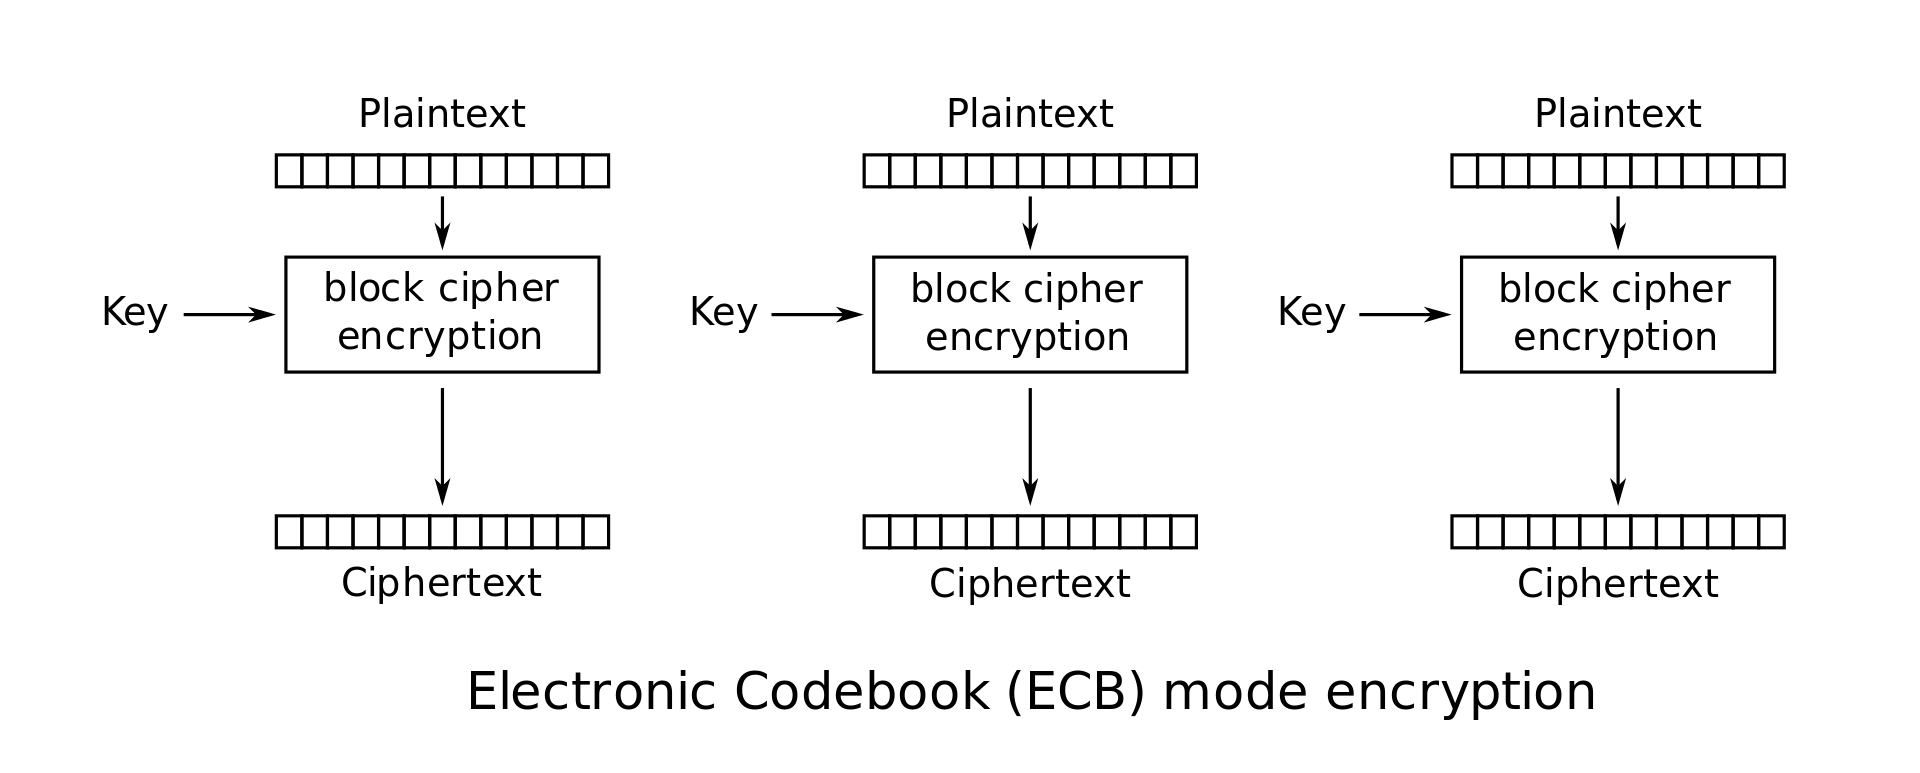
\includegraphics[width=0.5\textwidth]{figures/Ecb_encryption.png}
	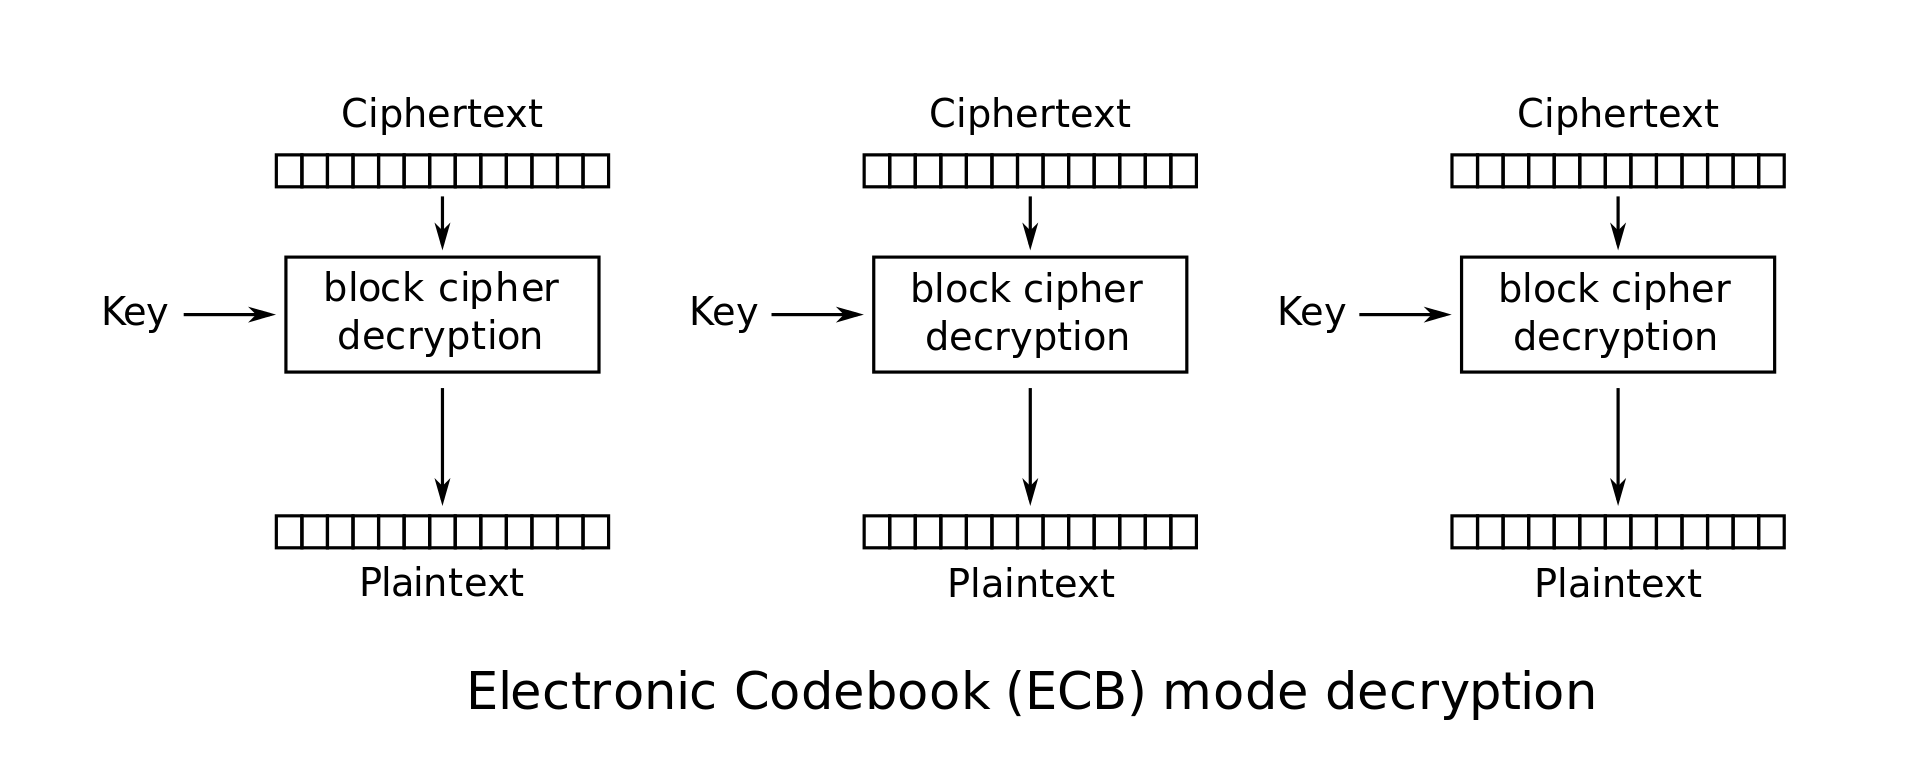
\includegraphics[width=0.5\textwidth]{figures/Ecb_decryption.png}\\
	$\Rightarrow$ the same plaintext block will result the same ciphertext block
	\paragraph{Cipher-Block Chaining (CBC)} .\\
	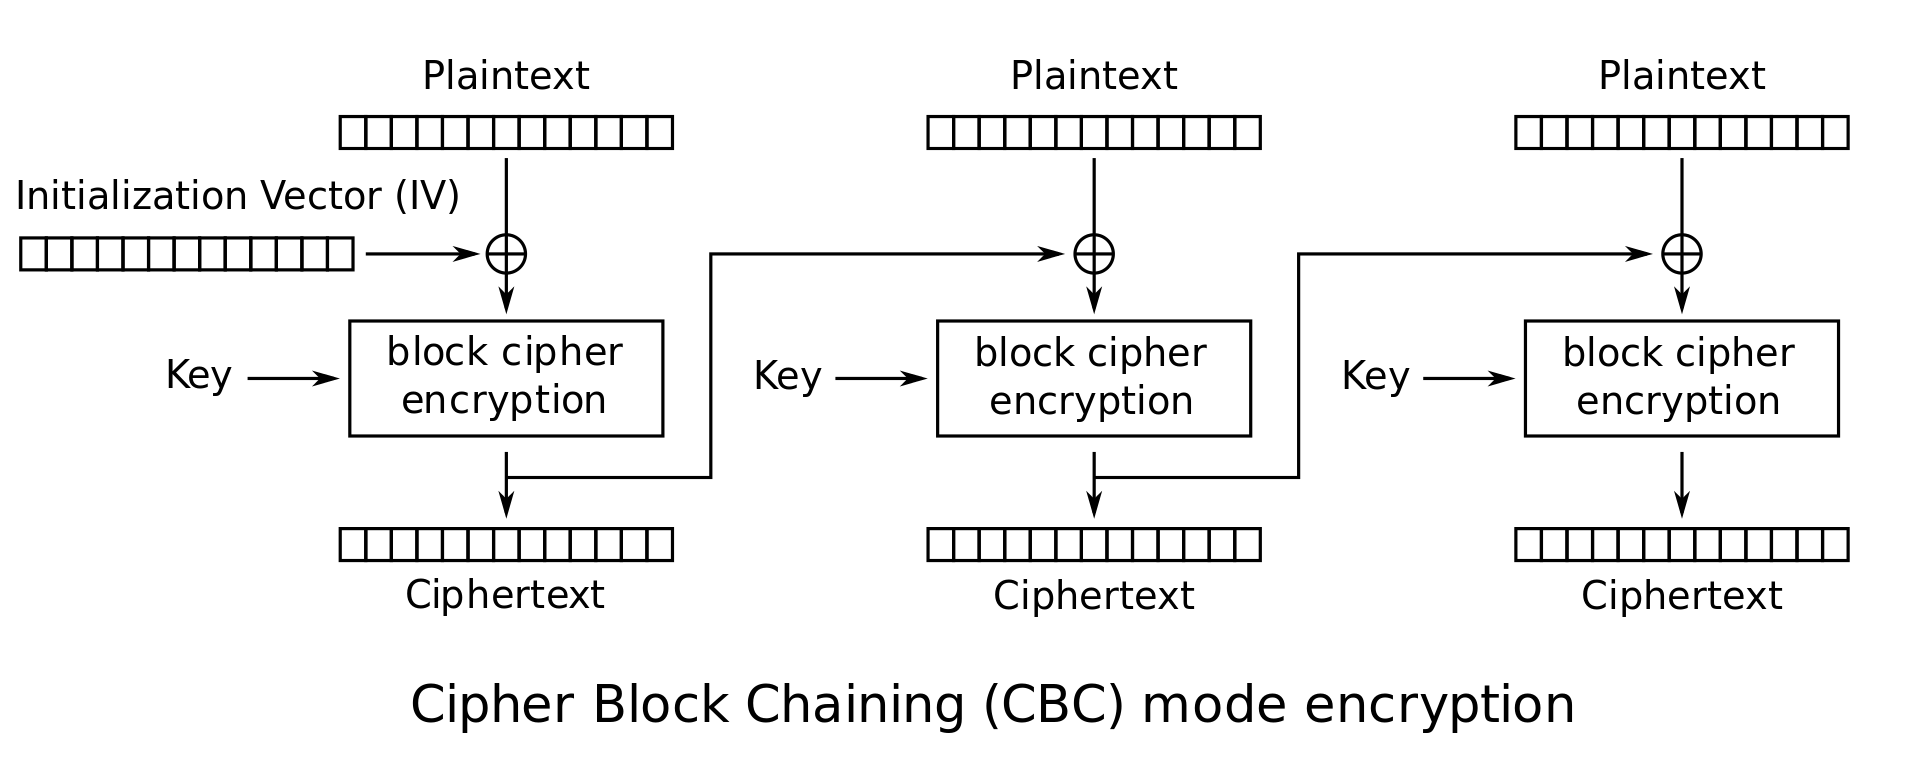
\includegraphics[width=0.5\textwidth]{figures/Cbc_encryption.png}
	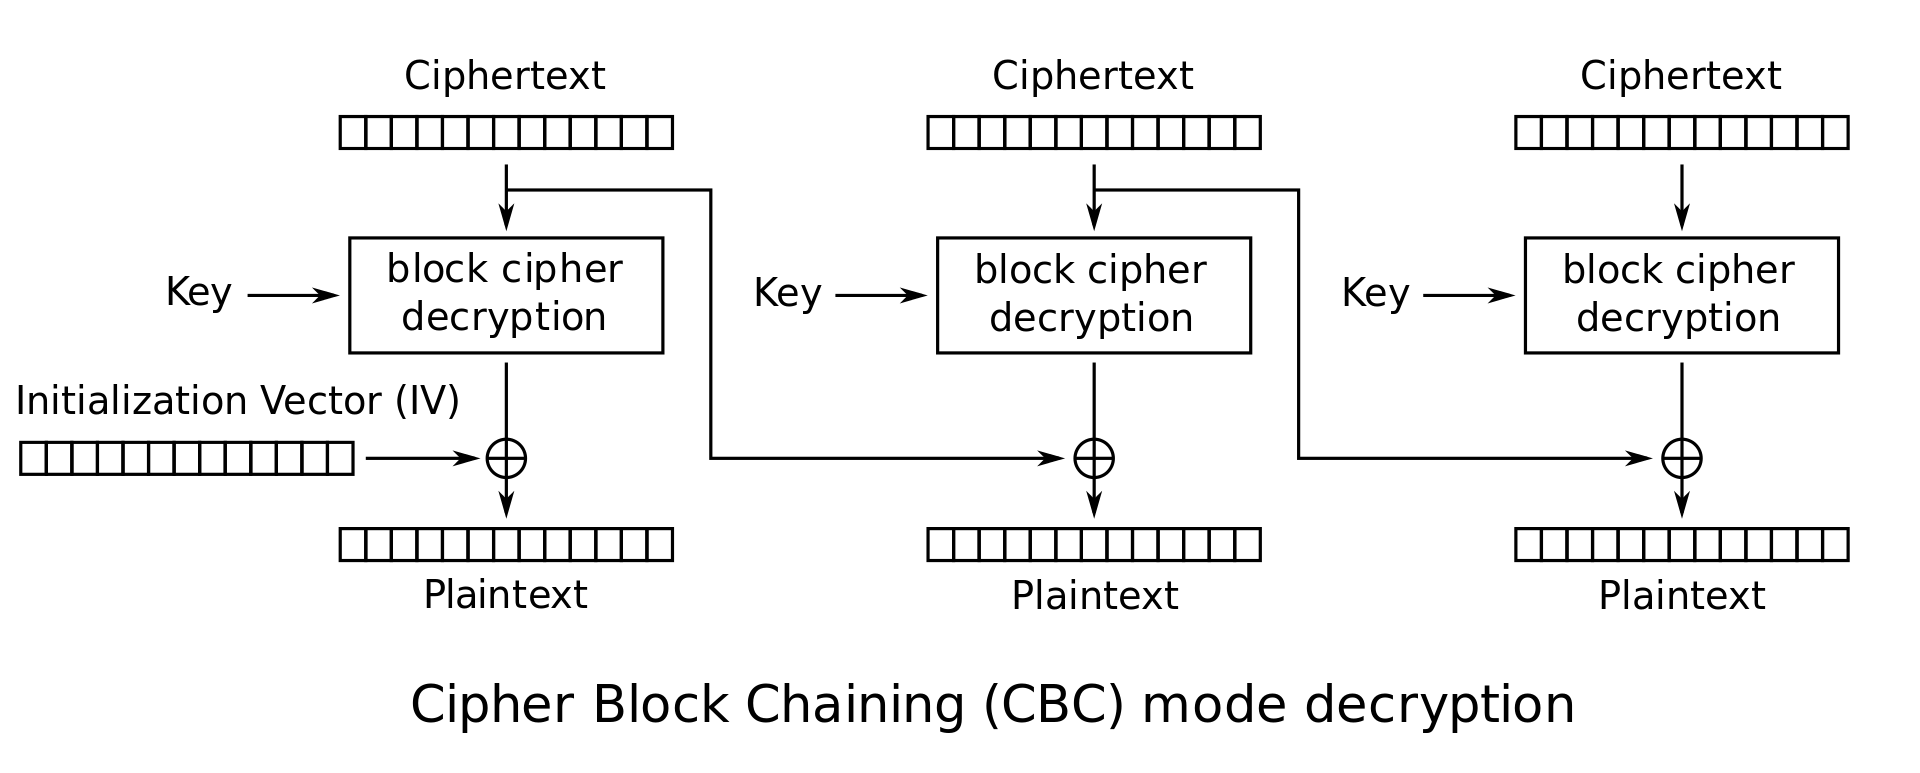
\includegraphics[width=0.5\textwidth]{figures/Cbc_decryption.png}
	\paragraph{Output Feedback Mode (OFB)} .\\
	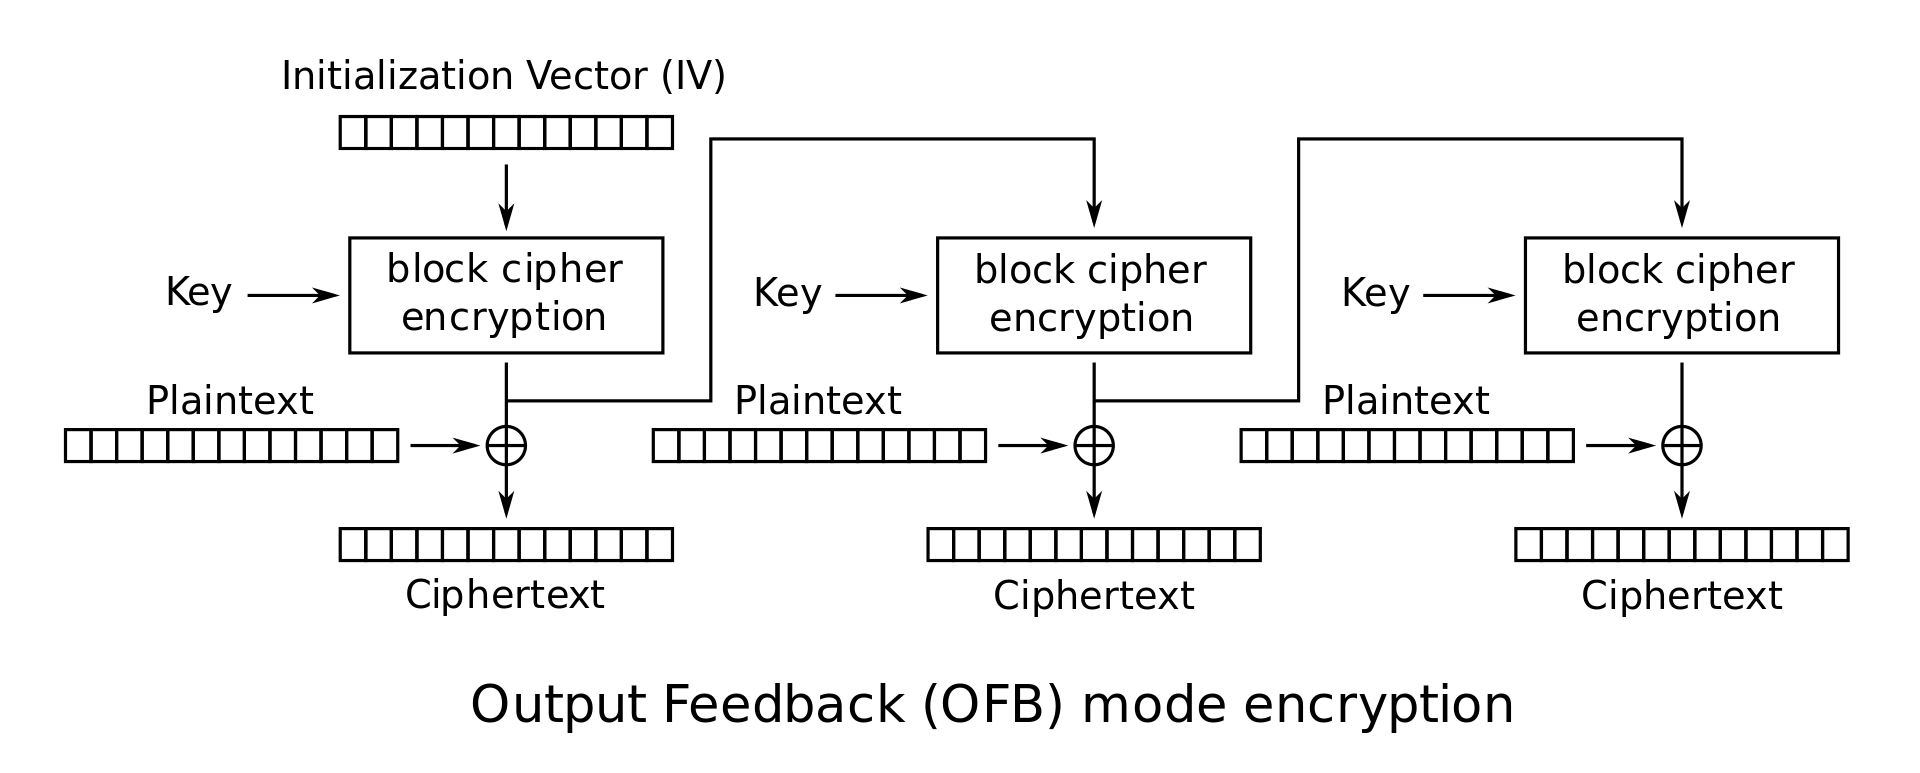
\includegraphics[width=0.5\textwidth]{figures/Ofb_encryption.png}
	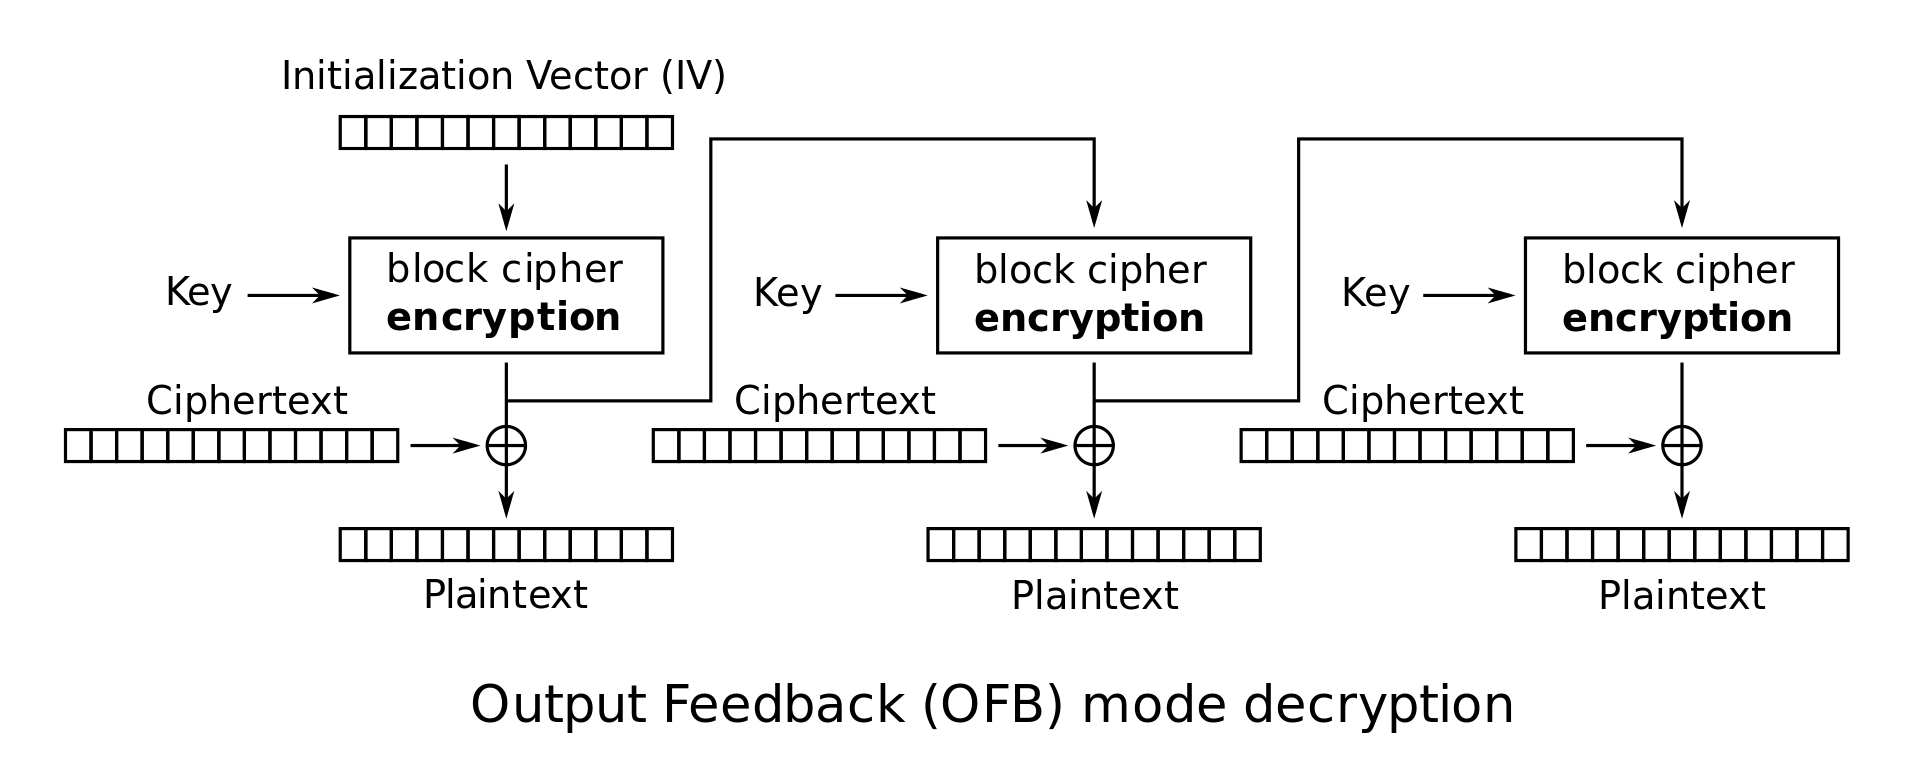
\includegraphics[width=0.5\textwidth]{figures/Ofb_decryption.png}
	\paragraph{Counter Mode (CTR)} .\\
	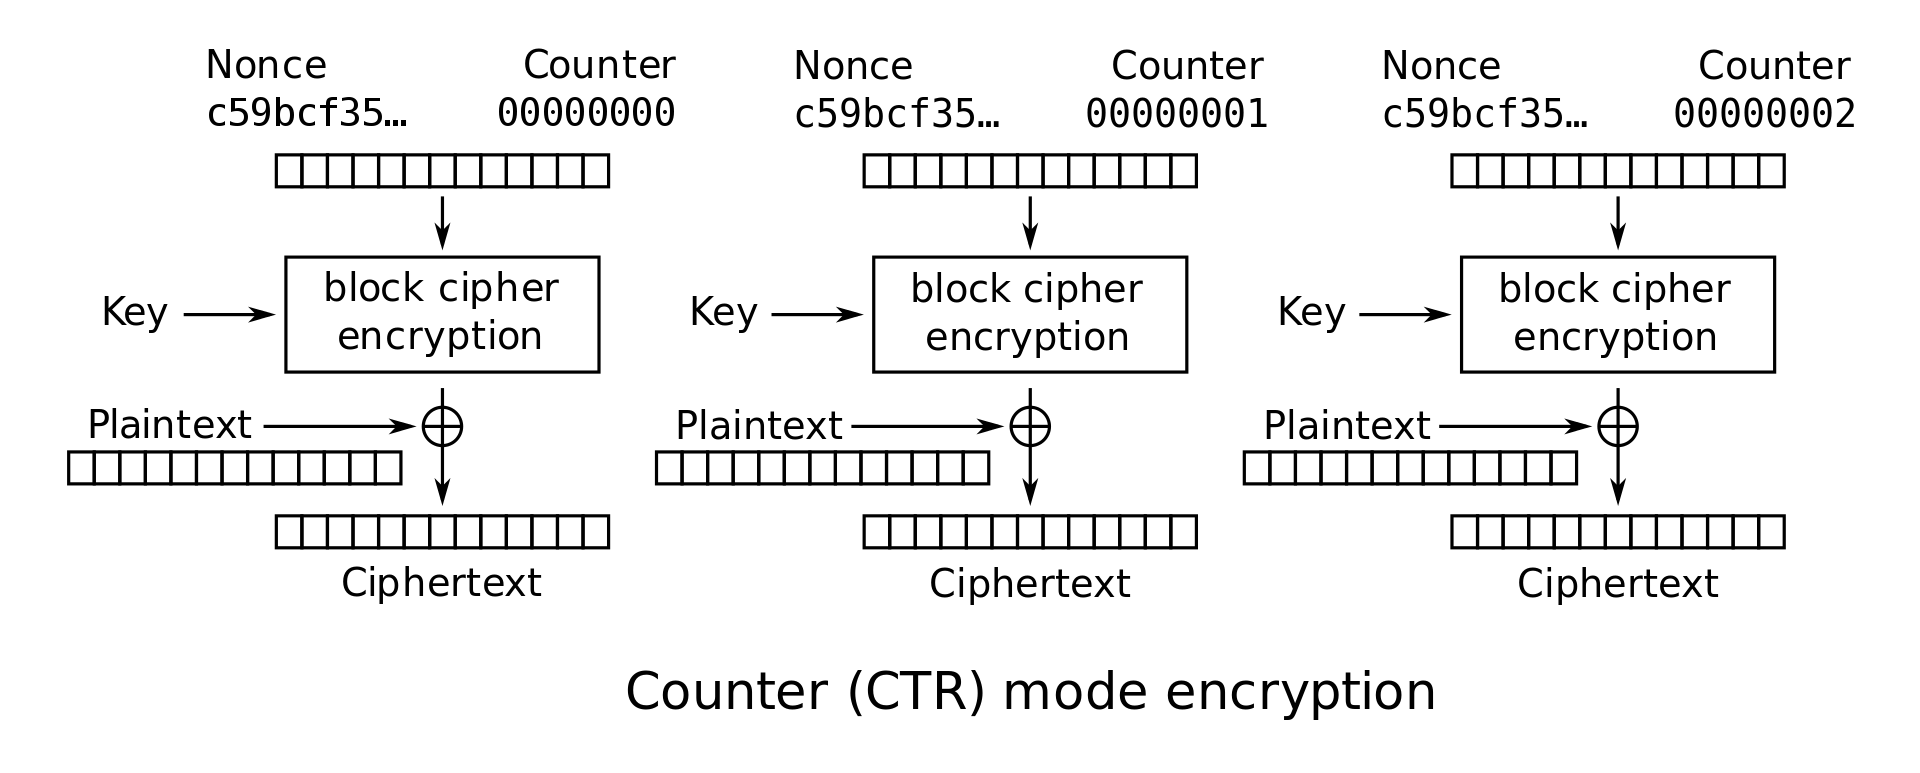
\includegraphics[width=0.5\textwidth]{figures/Ctr_encryption.png}
	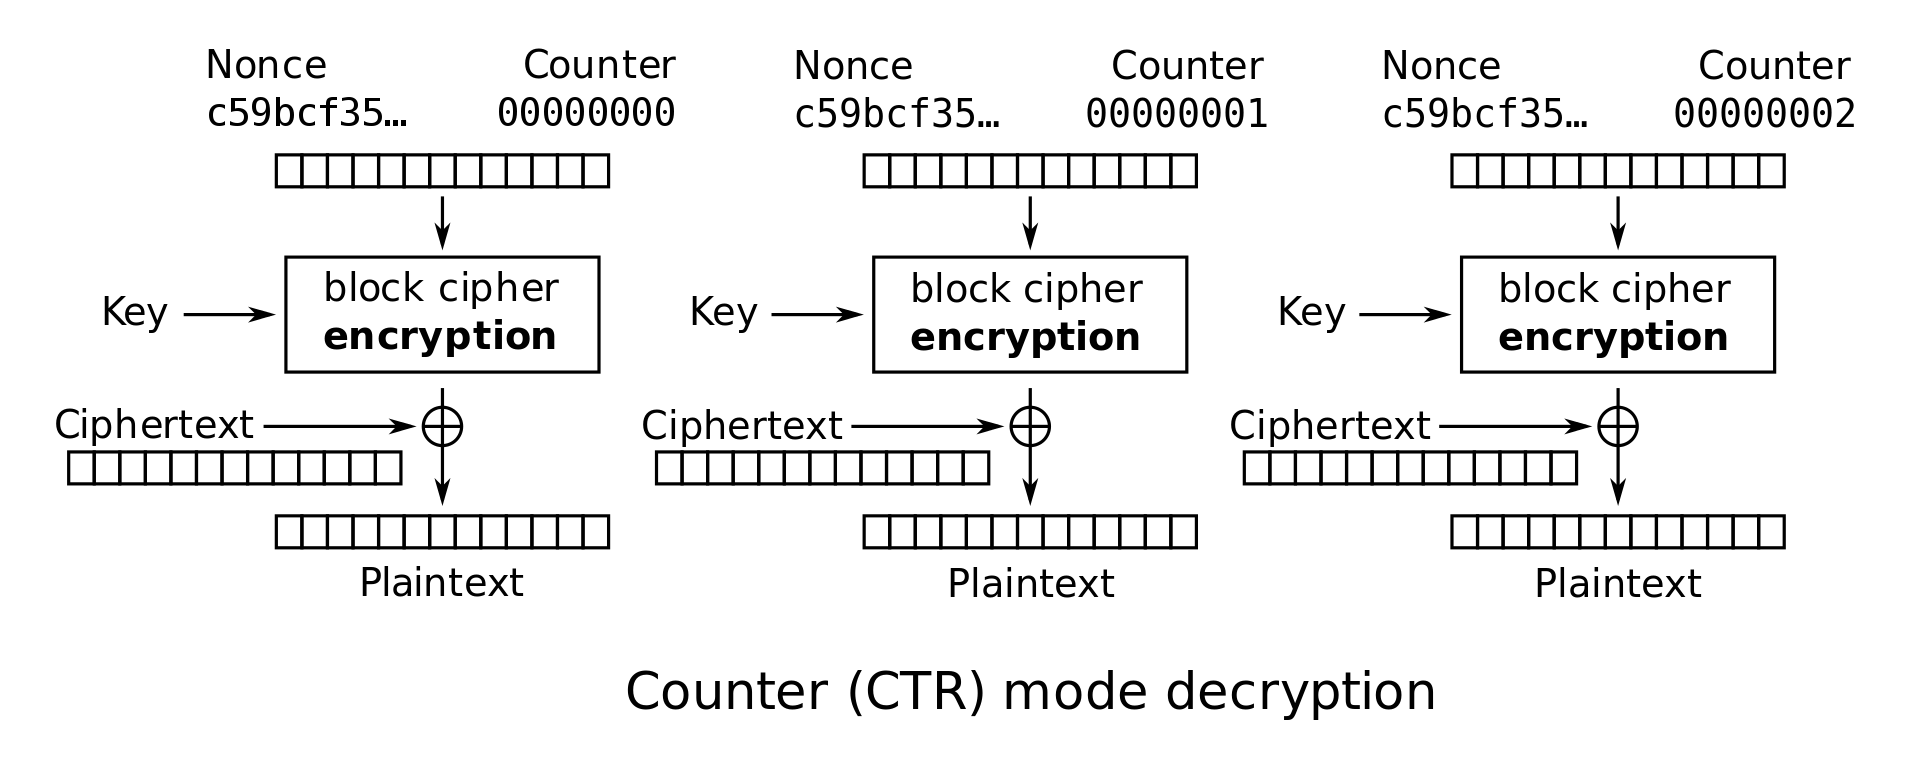
\includegraphics[width=0.5\textwidth]{figures/Ctr_decryption.png}
	
	\section{Message authentication}
	Ensure that a message is from a specified party and was not modified during transition.
	\textbf{Message authentication code (MAC) scheme} is a pair of tag ($Tag$) and verify ($Vrfy$) algorithm with $Vrfy_k(m,Tag_k(m)) = yes$ (tag is valid) for every plaintext message $m \in M$ plaintext space and key $k \in K$ key space. $Tag_k(m) = t$ generates a tag $t \in T$ set of tags. The verify algorithm just computes the tag again from the plaintext and compares the result with the given tag.\\
	$\rightarrow$ can be constructed from block ciphers (f.e. CBC-MAC) or hash functions\\
	\textbf{Replay attack} MACs do protect against the modification of the message through a third party but not against replaying an already delivered message with a valid tag again. Solution: time-stamps, sequence numbers, ...
	\textbf{Splicing attack} A CBC-MAC should be used with the message length $|m|$ as initialization vector (IV). Otherwise a splicing attack is possible:\\
	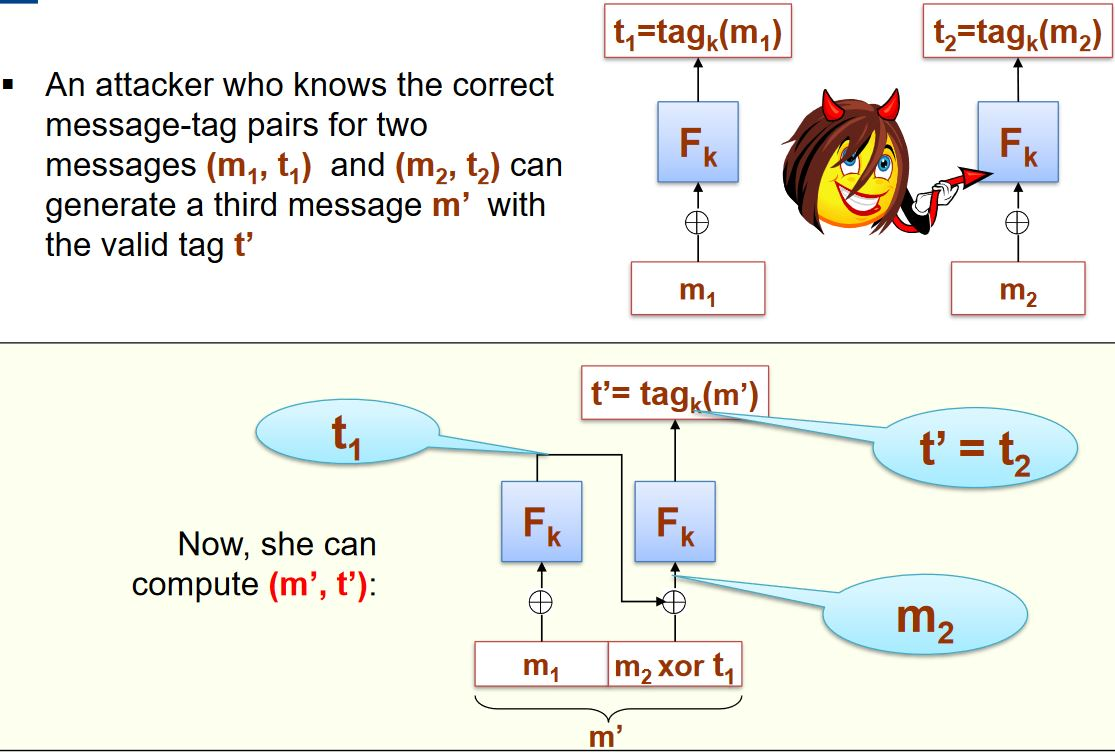
\includegraphics[width=\textwidth]{figures/splicing-attack.JPG}
	
	\subsection{Hash functions}
	Hash functions map arbitrary input to a fixed length of output. They should be collision resistant and one-way functions.(?)\\
	\textbf{Collision resistance} It's hard to find two inputs that have the same hash: $H(m) = H(m')$
	\textbf{Examples} of hash functions are MD5, SHA1, SHA2, SHA256, ...\\
	\textbf{HMAC} MAC based on a hash function: $HMAC_k(m) = H((k xor opad) || H(k xor ipad || m))$
	
	\subsection{Key distribution}
	\textbf{Key distribution center} There is an authority that all the users trust with its help it's possible to exchange session keys for direct communication. Not useful in the internet.\\
	${M}_K = Enc_{K0}(M), Tag_{K1}(Enc_{K0}(M))$ is a message $M$ that is encrypted and authenticated with key pair $K$.
	\textbf{Needham-Schroeder protocol} is a protocol for key exchange that prevents against reply and man-in-the-middle attacks (adversary can't reply the answer of the server because of the nonce, adversary can't manipulate message from Alice to Bob to change the identity who's sending the message)\\
	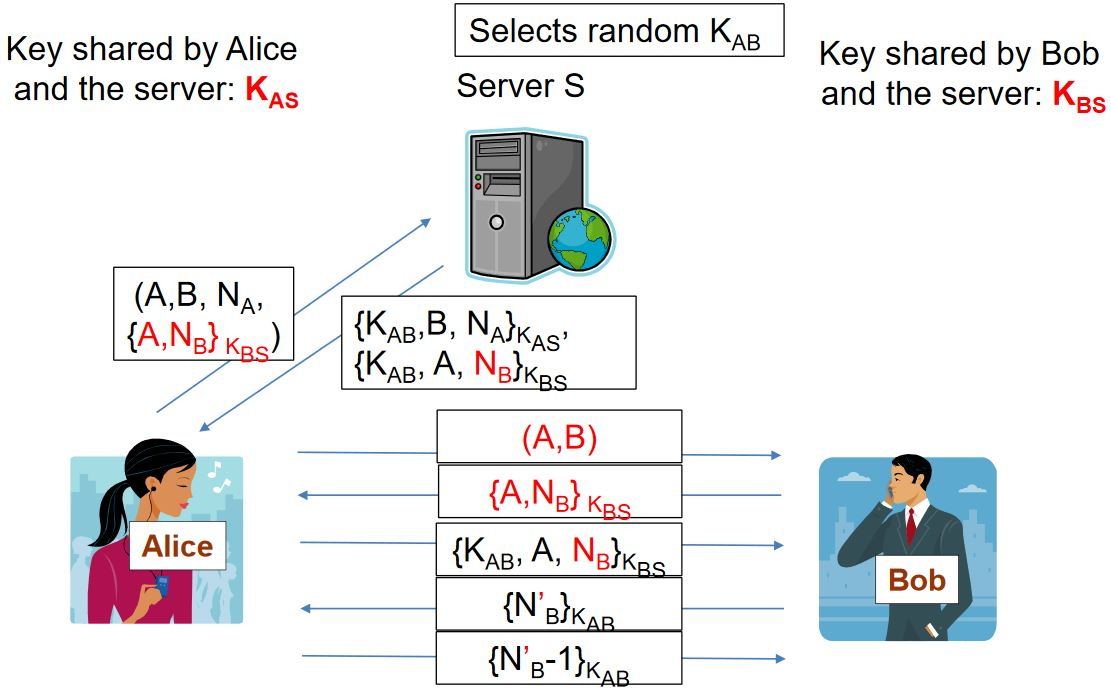
\includegraphics[width=\textwidth]{figures/needham-schroeder-protocol.JPG}\\
	\textbf{Peer-to-peer key distribution} can be achieved with public key cryptography
	
	\section{Public Key Cryptography}
	\paragraph{Encryption} Instead of using one key $k$, use a public key $pk$ for encryption and a private or secret key $sk$ for decryption.\\
	$\Rightarrow$ everyone can encrypt messages for the person who owns the private key because the encryption key is public
	\paragraph{Authentication} Use the private key to create a tag (also called signing a message) and the public key to validate the tag\\
	$\Rightarrow$ everyone can validate tags from the person who owns the private key. So signatures can be passed on and also be verified by a third party.
	\paragraph{Problems}
	\begin{itemize}
		\item how are the public keys exchanged?
		\item how to revoke keys?
	\end{itemize}
	
	\subsection{RSA algorithm}
	RSA is a trapdoor one-way function which can be inverted if a secret (the secret key) is known. The security relies on the hardness of the \textbf{factorization of large integers}.\\
	\textbf{Key generation} Generate large primes $p$, $q$ (1024 bits each is seen as secure $\rightarrow$ 2048 bit RSA)\\
	Compute $N=pq$ and $\varphi(N)=(p-1)(q-1)$, choose $e$ as co-prime to $\varphi(N)$, choose unique $d$ as inverse of $e \mod \varphi(N) \rightarrow ed = 1 \mod \varphi(N)$\\
	\textbf{Public key} = $(e,N)$, \textbf{private key} = $d$\\
	\textbf{Encryption} $c = m^e \mod N$\\
	\textbf{Decryption} $c^d \mod N = (m^e)^d \mod N = m$\\
	$\Rightarrow$ To be secure a (pseudo-)random padding is required so that the algorithm doesn't output the same ciphertext for the same plaintext.
	
	\subsection{Elgamal}
	Another public key cryptosystem which is based on the discrete logarithm hardness assumption.
	
	\subsection{Distribution of public keys}
	\textbf{Cerification Authority (CA)} signs certificates that hold the public key of a person and specify to which person it belongs. So everyone who has the public key of the CA and trusts it can verify the certificate.\\
	\textbf{Certificate Chain} CA certificates a person $P_1$ who can certificate another person $P_2$. A third person who trusts the CA and $P_1$ can now trust $P_2$. But \textbf{trust is not transitive}! CA must grant $P_1$ the right to certificate others (recommendation levels limit the length of the certification chain).\\
	\textbf{HTTPS/SSL} Root certificates that certificate a CA come with the browser and are build-in with recommendation level 1. So the browser trusts every certificate signed by the build-in CAs.
	
	\subsection{Diffie-Hellman key exchange}
	To encrypt the communication between two parties one key cryptography is used more often but the key is established using public key cryptography (for example HTTPS). This is because public key cryptography requires more computational power and is therefore slower. The Diffie-Hellman protocol is for exchanging new session keys for synchronous encryption. It relies on the hardness assumption of the difficulty of solving the \textbf{discrete logarithm problem (DLP)}.
	\begin{enumerate}
		\item choose prime $p$
		\item choose generator $g$ of $\mathbb{Z}_p^*$ (generator can compose every number in $\mathbb{Z}_p^* = x \mod p$ when multiplied with itself several times)
		\item Alice chooses random $x$ with $0 < x < p-2$ and calculates $h_1 = g^x \mod p$ and sends it to Bob
		\item Bob chooses random $y$ with $0 < y < p-2$ and calculates $h_2 = g^y \mod p$ and sends it to Alice
		\item the common key is $k = h_1^y \mod p = h_2^x \mod p = g^{xy} \mod p$
	\end{enumerate}
	$\Rightarrow$ because the logarithm in closed groups (discrete logarithm) is hard to compute this scheme is secure\\
	$\Rightarrow$ does not protect against man-in-the-middle attacks
	
	% TODO continue with lecture 06
	
	\end{document}
